\chapter{Literature Study}
\label{chp:litreview}
With our project objectives in mind, we review existing approaches to designing autonomous driving algorithms.
A taxonomy of the relevant literature is shown in Figure \ref{fig:lit_tax_sec}. 
The second layer of this figure reflect the architectures (the structure of the algorithm, its components and relationship between components) that can be used to design an autonomous driving algorithm.
These are the classical, end-to-end and partial end-to-end pipelines.

As described in the introduction, the classical pipeline uses a series of separate modules with unique functions to control the vehicle.
Two of these modules, trajectory planning and control, are relevant to this project and are discussed in more detail.
The end-to-end pipeline aims to use a neural network to perform the task of all the modules in the classical pipeline.
We categorise end-to-end approaches by the method used to train the neural network, namely reinforcement or imitation learning.
Finally, the partial end-to-end pipeline uses a neural network within the modularised structure of the classical pipeline. 
These approaches are categorised according to which function of the pipeline is learned by the neural network. 

\begin{figure}[htb!]
    \centering
    \input contents/chapt2/figs/literature_taxonomy_sections.tex
    \caption[A taxonomy of the autonomous racing literature with sections]{A taxonomy of the autonomous racing literature. The second layer reflects approaches to designing architectures, while the third row indicate techniques used within those architectures.}
    \label{fig:lit_tax_sec}
\end{figure}



\section{Classic Pipeline}
\label{sec:classic}

The driving software architecture used by classical approaches is split into an \emph{offline} and \emph{online} phase, as shown in Figure \ref{fig:full_stack}.
The offline phase occurs before the vehicle is deployed on the track.
If the track is known, then a global trajectory (also known as a \emph{raceline}) can be computed during this offline phase.
This raceline typically includes a path ($x(t), y(t)$) and velocity profile $v(t)$.

During the online phase, the vehicle is deployed onto and allowed to interact with a simulated or real track.
During this online phase, we are concerned with processing sensor input to generate control outputs.
The classical approach is to process the sensor data using a series of modules with well defined functions.
First, perception algorithms derive knowledge about the vehicles surroundings. 
This includes constructing an updated map, localising the vehicle within that map, and detecting obstacles such as other vehicles. 
A local planner then computes a local trajectory based on the current information provided by the perception module.
The local trajectory is similar to the raceline, except that it is has a shorter horizon.
Controllers then compute actuator commands that minimise the error between the actual and planned local trajectory.
We summarise approaches to trajectory planning and control due to their relevance to this project.

\begin{figure}[h]
    \centering
    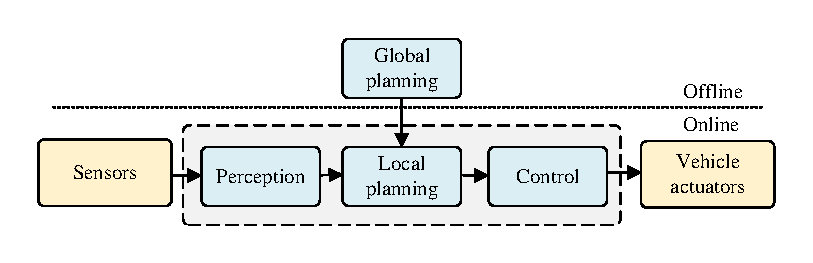
\includegraphics[width=\textwidth*8/10]{contents/chapt2/figs/classic_pipeline.png}
    \caption{The classic autonomous driving pipeline.}
    \label{fig:full_stack}
\end{figure}


\subsection{Local planning}
\label{sec:trajectory_planning}

Local trajectory planning is necessary because racing is a highly dynamic environment, especially when multiple vehicles are involved.
This means that global path may be infeasible or unsafe due to changing conditions on the track.
As such, a requirement for safe deployment of racing vehicles is to continually update a local trajectory according to the current track conditions.
The challenge for local planners is then to compute a trajectory faster than real-time.

Model Predictive Control (MPC) methods are the most commonly used and state of the art methods for local planning \cite{Betz2021}. 
This method relies on a vehicle dynamics model to optimise a finite horizon trajectory by minimising a specified cost function.
Only the first section of the trajectory is executed before optimising again.
MPC is powerful because it directly considers the vehicle and track constraints.
Therefore, so long as these constraints specified correctly, the trajectory generated is safe \cite{Schwenzer2021}.

The drawback to this method is that performing an optimisation at every time step is computationally expensive.
As such, many applications of MPC in autonomous racing, such as that by  Anderson et al. \cite{Anderson2016} and Funke et al. \cite{Funke2017} utilise simplified linear dynamics models that do not entirely capture the full non-linear system dynamics.
Despite the linearisation of dynamic models, computational expense may still result in the requirement for expensive hardware for online deployment \cite{Pan2017a}.
Furthermore, MPC relies on convexification (such as with quadratic approximation) of the cost function \cite{Williams2017}.

In summary, classical approaches have achieved impressive results owing to the use of optimisation techniques for planning and control. 
However, there are limitations to these optimisation techniques, such as the requirement for expensive computation (especially for non-linear dynamic models), expensive sensor suites due to the need for frequent and accurate state information, and lack of flexibility in the cost function. 
In particular, reliance on an accurate vehicle dynamics model is a serious issue due to the difficulty of measuring the model parameters \cite{Kabzan2019, Pan2017}.


%Global trajectory planning
%geometric
%\cite{Braghin2008} - shortest path vs minimum curvature

%optimisation
%\cite{Herrmann2019} - energy management
%\cite{Herrmann2020} - optimization includes power usage of battery

%genetic algorithms
%\cite{Cardamone2010}
%\cite{Vesel}

%Local trajectory planning
%\cite{Liniger2015a} - viability kernel for safe set of states
%\cite{keefer2022} 
%\cite{Wang2021}
%\cite{Jeon2013} - a* shortest path search


\subsection{Control}
\label{sec:control}

In the previous section, we described common methods of generating a local trajectory.
This local trajectory provides the reference information for \emph{lateral} and \emph{longitudinal} control commands, respectively.
These control commands are the steering angle $\delta$ for lateral control, and $a_{\text{long}}$ for longitudinal control, which are sent to low-level controllers for actuating the motors. 
We discuss several approaches falling into two broad categories of control: classic and MPC.

Classic controllers utilise well known principles in the fields of path and velocity tracking.
The most basic classic controllers are those that assume a kinematic vehicle model.
This type of vehicle model assumes slipping never occurs.
Under this assumption, control laws can be derived by considering only the geometric properties of the vehicle.
One such approach is the pure pursuit algorithm for lateral contol by Coultier \cite{Coulter_1992}. 
Pure pursuit calculates the steering angle the car should maintain to reach a target point on the path which is a fixed distance away from the vehicle.
Of course, this steering angle is only correct when tire slip does not occur.

A classic approach that relaxes the no slipping assumption of pure pursuit is the Stanley controller by Hoffman et al. \cite{Hoffmann2007}.
This controller calculates the steering angle with a control law utilising the cross track and heading error.
These are the distance between the closest point on the path to the front axle of the vehicle, and the the angle between the heading of the vehicle and the tangent on the closest point on the path, respectively.
The longitudinal control action is computed using a proportional integral (PI) controller.




Classical approaches have achieved impressive results owing to the use of optimisation techniques for planning and control. 
However, there are limitations to these optimisation techniques, such as the requirement for expensive computation (especially for non-linear dynamic models), expensive sensor suites due to the need for frequent and accurate state information, and lack of flexibility in the cost function. 
In particular, reliance on an accurate vehicle dynamics model is a serious issue due to the difficulty of measuring the model parameters \cite{Kabzan2019, Pan2017}.

%latitude and longitude control
%\cite{Kritayakirana2010} gg diagram control
%model predictive controllers
%\cite{Pup2020} - characterising uncertainty in vehicle models from linearisation
%\cite{Beal2013} - vehicle stabilisation at limits of handling
%\cite{Liniger2019} - viability kernel to limit search space
%\cite{Williams2016} - model predictive path integral control  
%\cite{Hewing2018} - control cars under model inaccuracy with learning non-linear mpc

%\subsection{Full driving stacks}
%\label{sec:full_driving_stacks}
%\cite{Valls2018}
%\cite{sherif2020}
%\cite{Wischnewski2019} - kinematic state estimation
%\cite{Vazquez2020} - in global planning
%\cite{alvarez2022}

\section{End-to-end pipeline}
\label{sec:end_to_end}

The limitations of classical methods has led to research in learning-based systems that improve the vehicle dynamics model or action policy with real-world data and allow more complex cost formulations and non-linear dynamics \cite{Fuchs2021}.
Many learning approaches use an end-to-end pipeline, illustrated in Figure \ref{fig:end_to_end}, whereby a single neural network predicts control outputs from sensor data.
The neural networks used in end-to-end approaches are typically trained using imitation or reinforcement learning paradigms \cite{Betz2021}. We present a summary of research efforts into both approaches.

\begin{figure}[h]
    \centering
    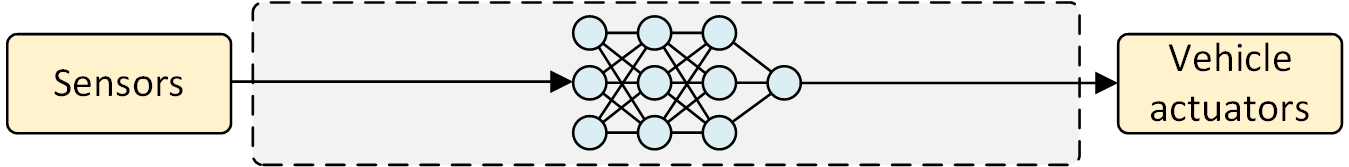
\includegraphics[width=\textwidth*8/10]{contents/chapt2/figs/end_to_end_pipeline.png}
    \caption{The end-to-end autonomous driving pipeline.}
    \label{fig:end_to_end}
\end{figure}

\subsection{Imitation learning}
\label{sec:imitation_learning}

Imitation learning techniques train a neural network to mimic an expert such as a human or optimisation method.
The process is analogous to supervised learning, where labelled data is used to train an algorithm to predict outcomes on new data.
In the context of autonomous racing, the labelled training data is produced by allowing an optimisation method or human to interact with the vehicle.
This produces a set of control commands which act as the labels for the inputs to the neural network.
Supervised learning is then used to train an algorithm to predict control commands for new data \cite{Osa_2018}.


Imitation learning is a good choice for training a neural network if it is feasible for an expert to demonstrate optimal behaviour, but difficult to define a reward manually.
For instance, in some circumstances where vehicle manoeuvres are complex, correct driving behaviour may be more easily specified by a human demonstrator than manually designing a reward signal.
Furthermore, the expert limits the need for exploration, resulting in faster and safer policy convergence than with reinforcement learning, which requires exploration \cite{Osa_2018}.


Many approaches, such as those by Tatulea-Codrean et al. \cite{Tatulea-Codrean2020}, Pan et al. \cite{Pan2017a} and Lee et al. \cite{lee2019} rely on a variant of the MPC algorithm from classical methods for expert training data. 
As such, the link between classical and end-to-end imitation learning approaches is stronger than for classical and end-to-end reinforcement learning approaches.
This makes the benefits of using a neural network over classical methods clearer in the imitation learning literature than reinforcement learning literature.

A major benefit of imitation learning with neural networks is the cost of online computation: neural networks are far less computationally expensive to run than optimisation methods. This is demonstrated by Tatulea-Codrean et al. \cite{Tatulea-Codrean2020}, who train a neural network to mimic the policy of a non-linear MPC (NMPC). The NMPC is too computationally expensive for real-time control of the vehicle. 
However, the neural network computes the control command in a much faster time, enabling the deployment of the vehicle.

Imitation learning in conjunction with neural networks also have the benefit of being flexible towards their inputs. 
Optimisation methods have strict requirements for the input as frequent state and boundary condition updates, a neural network is able to learn from high dimensional inputs such as images from a video feed. 
This is accomplished by Mahmoud et al. \cite{Mahmoud2020} and Pan et al. \cite{Pan2017a}. 
Pan et al. \cite{Pan2017a} showcase the usefulness of this property by using imitation learning to relax hardware requirements and reduce the cost of the vehicle sensor suit. 
Their neural network is trained to mimic an MPC on a vehicle with two sensor suits: an IMU and GPS unit worth 6000\$, and 500\$ camera.
While the MPC requires the 6000\$ IMU and GPS, the neural network is trained to execute the same policy on the 500\$ camera.

The flexibility of neural networks towards their inputs is related to another useful property: robustness to sensor noise and failure. 
This property is showcased well by Lee et al. \cite{lee2019}, who use imitation learning to create an ensemble of bayesian neural networks (BNN) on different sensor inputs to create a redundant control policy. 
The algorithm is robust to sensor noise and even multiple sensor failures, which was not possible using more traditional optimisation methods.

From these examples we see that imitation learning learning with neural networks is a powerful tool.
However, Wadekar et al. \cite{Wadekar2021} highlight some weaknesses of the imitation learning technique.
The neural network policy will not match the expert policy exactly. 
Since policy affects the distribution of states that the vehicle encounters, the vehicle may encounter a scenario for which no expert training data was generated during training, in which case it is likely to take an incorrect action \cite{Osa_2018}.
Furthermore, Wadekar et al. \cite{Wadekar2021} describe that the data collected by the expert must be curated so that the agent does not learn any undesirable behaviour.
Perhaps the most undesirable characteristic of imitation learning is that it requires expert training data.
This makes it unsuitable for scenarios where expert training data is not available, as in cases where optimisation methods fail \cite{Fuchs2021a}.
As such, we turn towards a method for training neural networks for control tasks that does not require expert training data.

\subsection{Reinforcement learning}
\label{sec:reinforcement_learning}

Reinforcement learning optimises a neural network policy to maximise a scalar reward signal through direct interaction with the environment \cite{Plaat_2022}. 
The benefits of using reinforcement learning are the same as the imitation learning approach, i.e., less stringent sensor requirements, robustness to sensor failure, and fast online execution time. However, the technique allows for more complex cost formulation than what is possible with even state of the art expert optimisation methods and negates the need for expert training data \cite{Fuchs2021}.
%Reinforcement learning approaches may be categorized according to their action selection method. Whereas model-based methods use a model of the vehicle and environment to plan ahead, model-free methods select an action based only on past experience. 


Several research efforts into reinforcement learning applied to autonomous racing have been aimed at creating pixel to control algorithms. 
Perot et al. \cite{Perot2017} and Jaritz et al. \cite{Jaritz2018} are early works in model-free reinforcement learning applied to autonomous racing that present such pixel to control algorithms for racing in the video game World Rally Cross 6.
Both approaches utilise a convolutional neural network (CNN) with long short-term memeory (LSTM). 
Jaritz et al. \cite{Jaritz2018} state that a score given at the end of the race is too sparse for the agent to learn effectively.
They therefore introduce a continuous reward schema.
Continuous reward schemas have been used by every approach reviewed since Perot et al. \cite{Perot2017} and Jaritz et al. \cite{Jaritz2018}.
However, the approaches show that pixel to control is both extremely inefficient, as both Jaritz et al. \cite{Jaritz2018} and Perot et al. \cite{Perot2017} train their agent for 80 million steps.



Another pixel to control strategy is developed by Schwarting et al. \cite{Schwarting2021}, who apply model-based reinforcement learning to openAI gym's two player racecar environment.
When multiple vehicles are involved, the opponents behaviour must be taken into account.
However, these behavioral and environmental features may be too complex to be captured by MPC or purely game-theoretic approaches that assume perfect knowledge of the state of all vehicles.
Schwarting et al. \cite{Schwarting2021} showcase the strength of reinforcement learning to generate policies without perfect knowledge of the environment.
Their solution learns a model of the world (including the opponent behaviour) using a neural network.
This model is then used to generate imagined gameplay experiences to train the agent on.


A more recent and state of the art approach is presented by Fuchs et al. \cite{Fuchs2021}, who creates a model-free soft actor-critic (SAC) agent that achieves lap times on par with competitive e-sports drivers in the racing game Gran Turismo Sport.
Key to their approach is careful selection of hand-crafted input features that include: 1) the vehicles velocity $\pmb{v}_t \in \mathbb{R}^3$, 2) acceleration $\pmb{\dot{v}}_t \in \mathbb{R}^3$, 3) distance measurements of $M$ rangefinders $\pmb{d}_t \in \mathbb{R}^M$, 4) the previous steering command $\delta_{t-1}$, 5) a binary flag indicating wall contact, and 6) $N$ sampled curvature measurements of the track centerline $\pmb{c}_t \in \mathbb{R}^N$.
These are important input features, as most other reinforcement learning approaches that do not utilise a pixel to control strategy use a selection of these features as input to their neural network.
Fuchs et al. \cite{Fuchs2021} also introduce a continuous progress term into the reward signal, while penalising the agent for making contact with the track boundary:
\begin{equation}
    r_t = r_{t}^{\text{progress}} - 
    \begin{cases}
    c_w \| \pmb{v}_t \| & \text{if in contact with wall} \\
    0 & \text{otherwise}
    \end{cases}
\end{equation}
where $c_w$ is a tuned constant.
Although their implementation remains in simulation, Fuchs et al. \cite{Fuchs2021} do measure the effect of vehicle model inaccuracies by changing the parameters of the vehicle model between training and testing. They find that increased tire friction causes the agent to steer more aggressively leading to brief contact with the inside wall. A decrease in tire friction causes the agent to take corners slightly wide resulting in contact with the outside.
They also measure the effect of delays to the agents inference, finding that delays of greater than 100ms leads to track boundary contact. 
However, it is not clear from Fuchs et al. \cite{Fuchs2021} what degree of model inaccuracy results in collisions.


Song et al. \cite{Song2021} extends the work from Fuchs et al. \cite{Fuchs2021} to a multi-agent setting, training an agent to overtake other vehicles in Gran Turismo Sport.
key to their success is the use of curriculum learning, whereby the agent is trained to solve increasingly difficult tasks by adding components to both the environment and reward signal. 
The agent is trained to race on its own before another vehicle is added to the simulation, and the reward signal is modified to encourage the agent to make progress relative to the other vehicle.
This showcases the strength of reinforcement learning over optimisation methods: while optimisation algorithms rely on the convexification of cost functions, reinforcement learning agents can learn to solve difficult tasks from complex cost functions.


We now move away from now games and discuss research efforts that more directly address the sim2real gap and deployment onto physical cars.
Niu et al. \cite{Niu2020} anticipate that the reinforcement learning algorithm may select an unsafe action.
To prevent this, they propose a model-based safety controller that acts as a safeguard mechanism to prevent the agent from selecting unsafe actions.
Furthermore, they foresee that the safety module's reliance on an accurate vehicle model presents an issue. 
As such, a neural network is used to learn a vehicle model online that eventually replaces the initial assumed vehicle model.
This idea of improving a vehicle model after the vehicle is deployed is a commonplace sim2real practice.
Another benefit of the safety controller is that it constricts the agent's exploration, allowing the policy to converge faster and more robustly.


Another issue that presents itself during physical deployment is that of control smoothness. 
Sudden control actions will induce excessive mechanical wear and cause the vehicle to exhibit dangerous behaviour.
Hsu et al. \cite{hsu2022} identify this issue andapply Conditioning for Action Policy Smoothness (CAPS) to smooth the control action of the vehicle.
Although Hsu et al. \cite{hsu2022} do not directly address model inaccuracies, their policy smoothing approach produces a conservative policy which is expected to increase performance and safety in settings where the model inaccuracies occur.
This is because a smoother policy results in less lateral and longitudinal acceleration and does not bring the vehicle as close to its handling limits as a jerkier policy.


More sim2real practices are explored by Chisari et al. \cite{Chisari2021}, who deploy a soft actor-critic model-free reinforcement learning algorithm onto a physical vehicle.
They make the agent policy robust to real-world transfer training in simulation with a slightly randomised vehicle model.
The agent policy is then refined by retraining the neural network after the physical vehicle is deployed.
This allows the reinforcement learning algorithms to achieve lap times but have the number of track boundary collisions as an MPC controller.
Ivanov et al. \cite{Ivanov2020} take a similar approach to Chisari et al. \cite{Chisari2021} by training an agent with model randomisation, but are not able to achieve robustness to the sim2real transfer.


The final end-to-end approach we discuss is by Brunbauer et al. \cite{brunnbauer}, who demonstrate demonstrate the effectiveness of advanced model- based deep RL compared to model-free agents in the real-world application of autonomous racing.
Brunnbauer et al. \cite{brunnbauer} deploy the model-based Dreamer reinforcement learning algorithm by Hafner et al. \cite{Hafner2019a} on a physical F1tenth vehicle.
Their algorithm learns an observation model which is used to predict agent-environemnt interactions.
It then learns a policy purely on imagined sequences using the observation model, without interaction with the environment.
This results in safe and data-efficient learning.

\begin{landscape}
    \newcolumntype{a}{>{\hsize=1\hsize \centering\arraybackslash}X}
\newcolumntype{d}{>{\hsize=.5\hsize \centering\arraybackslash}X}
\newcolumntype{e}{>{\hsize=2\hsize \centering\arraybackslash}X}


\begin{table}[h]
\centering
\begin{tabularx}{21cm}{|a|d|d|d|d|e|}
    
    \hline
    \small \textbf{Name} & \small \textbf{Model-based} & \small \textbf{Multi-agent} & \small \textbf{Input} & \small \textbf{Physical vehicle} & \small \textbf{sim2real approach} \\
    \hline
    \small Schwarting et al. \cite{Schwarting2021} & \checkmark & \checkmark & \small game image & & - \\
    \hline
    \small Brunnbauer et al. \cite{brunnbauer2021} & \checkmark & & \small features & \checkmark & - \\
    \hline
    \small Perot et al. \cite{Perot2017} & & & \small game image & & - \\
    \hline
    \small Jaritz et al.  \cite{Jaritz2018} & & & \small game image & & - \\
    \hline 
    \small Fuchs et al. \cite{Fuchs2021} & & & \small features & & \small Test effects of model inaccuracy in simulation \\
    \hline
    \small Remonda et al. \cite{Remonda2021} & & & \small features & \checkmark & - \\
    \hline 
    \small Song et al. \cite{Song2021} & & \checkmark & \small features & & - \\
    \hline
    \small Niu et al. \cite{Niu2020} & & & \small features & & \small Safety module based on learned vehicle model prevents agent from selecting unsafe actions. \\
    \hline
    \small Chisari et al. \cite{Chisari2021} & & & \small features & \checkmark & \small Parameter randomisation while training, policy refinement after deployment \\
    \hline
    \small Ivanov et al. \cite{Ivanov2020} & & & \small features & \checkmark & \small Parameter randomisation while training \\
    \hline
    \small Hsu et al. \cite{hsu2022} & & & \small image & \checkmark & \small Control action smoothing \\
    \hline

\end{tabularx}
\caption[A summary of end-to-end reinforcement learning approaches for autonomous racing]{A summary of end-to-end reinforcement learning approaches for autonomous racing.}
\label{table:autonomous_racing_rl_summary}
\end{table} 

    \footnote{The absence of a tick in the model-based, multi-agent , and physical vehicle columns indicate that the approach was model-free, single-agent and simulation only, respectively. \label{footnote_1}}
\end{landscape}



\section{Partial end-to-end pipeline}
\label{sec:partial_end_to_end}

Wrapping the entirety of the driving task into one neural network has repercussions.
As the neural network needs to learn all three high level tasks from the classical pipeline (perception, planning and control), it can overfit the training data, leading to suboptimal policies.
Betz et al. and \cite{Weiss2020} et al. \cite{Betz2021} argue that it would be simpler to learn only one task from the classic pipeline.
Furthermore, Weiss et al. \cite{Weiss2020} argue that even though end-to-end methods perform well on validation data, that does not mean that the method contains a useful driving strategy that can perform well in an actual driving test.
This is because end-to-end methods fail to capture how expert drivers behave.
Expert drivers do not select only the control action at the current time step based on their current vehicle state, but instead plan out a trajectory. 
They then execute control commands to achieve that trajectory.
Furthermore, slight errors in the control input can lead to very large errors in the trajectory, resulting in catastrophe.

We therefore consider the approach that synthesises the classic and end-to-end pipelines by learning a section of the classic pipeline with a neural network. 
This is known as the partial end-to-end pipeline.
There are two possible architectures within the partial end-to-end pipeline: either the trajectory planner or the controller is learned using a neural network. 
These two architectures are shown in Figure \ref{fig:pete}.
We now give attention to research efforts the partial end-to-end pipeline.

\begin{figure}[h]
    \centering
    \begin{subfigure}[htb!]{\textwidth}
        \centering
        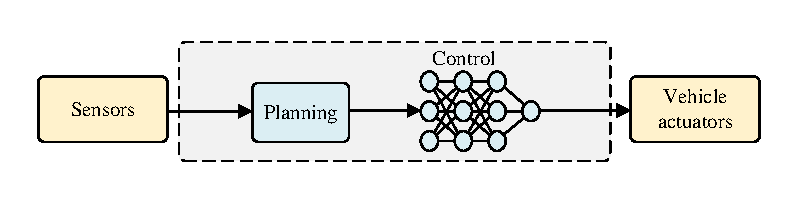
\includegraphics[width=\textwidth*8/10]{contents/chapt2/figs/partial_end_to_end_pipeline_learned_control.png}
         \caption[The partial end-to-end pipeline with a learned controller]{The partial end-to-end pipeline with a learned controller.}
        \label{fig:pete_learned_control}
    \end{subfigure}
    \hfill
    \begin{subfigure}[htb!]{\textwidth}
        \centering
        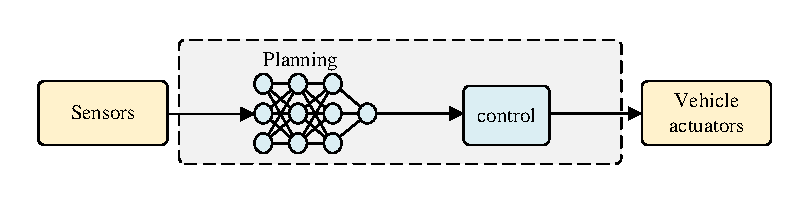
\includegraphics[width=\textwidth*8/10]{contents/chapt2/figs/partial_end_to_end_pipeline_learned_trajecory_planning.png}
        \caption[The partial end-to-end pipeline with a learned trajectory planner]{The partial end-to-end pipeline with a learned trajectory planner.}
        \label{fig:pete_learned_trajectory_planning}
    \end{subfigure}
\caption[Configurations of the partial end-to-end pipeline]{The two configurations of the partial end-to-end pipeline.}
\label{fig:pete}
\end{figure}

\subsection{Learned controller}
\label{sec:learned_controller}
We first consider approaches where the control task is learned by a neural network, as shown in Figure \ref{fig:pete_learned_control}.

Evans et al. \cite{Evans2021b} trained a reinforcement learning agent to modify control commands from a pure pursuit path follower that tracks a global plan.
The agent is trained to modify the control input to avoid randomly placed obstacles.
Evans et al. \cite{Evans2021b} measure similar performance for both the end-to-end and partial-end-to-end method.
However, a kinetic bicycle model that does not account for tire slipping is used.

Rather than learn only part of the control task, Ghignone et al. \cite{Ghignone2022} replace the entire controller with a reinforcement learning agent.
The agent is trained with varying tire friction coefficients to generalise to different model parameters.
Their agent outperforms both the MPC and end-to-end baseline by a large margin under model mismatch conditions.

The disadvantage to this method is that even though a reference path is computed, the control action is still given by a neural network.
Furthermore, since trajectory planners from classical methods are used, this architecture suffers from the same drawbacks as described in section \ref{sec:trajectory_planning}.

\subsection{Learned Trajectory planner}
\label{sec:learned_planner}
We now discuss approaches where the control task is learned by a neural network. This architecture is shown in Figure \ref{fig:pete_learned_trajectory_planning}.

Weiss et al. \cite{Weiss2020a} train an imitation learning agent to generate a local path as a bezier curve.
A pure pursuit controller is used to ensure that the vehicle tracks this path.
The approach outperformed end-to-end approaches in terms of distance races and generalisation across different tracks.
However, model uncertainty is unaccounted for.
A similar approach is taken by Capo et al. \cite{Capo2020}, except that a reinforcement learning agent outputs only a single point in front of the vehicle, which is tracked using low-level logic.
The approach outperformed end-to-end approaches in terms of distance races and generalisation across different tracks. However, similarly to Weiss et al. \cite{Weiss2020}, they do not take model uncertainty into account.


All partial end-to-end pipeline results indicate that the partial end-to-end pipeline outperforms the end-to-end pipeline.

\newcolumntype{R}{>{\raggedleft\arraybackslash}p{2.7cm}}
\newcolumntype{M}{>{\centering\arraybackslash}p{1.8cm}}
\newcolumntype{N}{>{\centering\arraybackslash}p{2.2cm}}
\newcolumntype{Y}{>{\centering\arraybackslash}p{1cm}}
\newcolumntype{L}{>{\raggedright\arraybackslash}p{4.5cm}}

\begin{table}[htb!]
\centering
\small
\renewcommand{\arraystretch}{1.1}
\begin{tabularx}{0.9\textwidth}{RYMNL}
    \hline
    \small \textbf{Author(s)} &  \small \textbf{Year} & \small \textbf{Learning method} & \small \textbf{Learned component} & \small \textbf{sim2real approach} \\
    \hline
    \small Weiss and Behl \cite{Weiss2020, Weiss2020a, Weiss2022} & \small $2020$ & \small IL & \small Planner  & - \\
    \small Capo et al. \cite{Capo2020} & \small $2022$ & \small RL &  \small Planner & - \\
    % \small Mahmoud et al. \cite{Mahmoud2020} & \small $2020$ & \small RL & \checkmark & & - \\
    \small Evans et al. \cite{Evans2021b} & \small $2021$ & \small RL &  \small Controller & - \\
    \small Ghignone et al. \cite{Ghignone2022} & \small $2022$ & \small RL &  \small Controller  & \small Randomise vehicle model parameters while training \\
    \hline
\end{tabularx}
\caption[A summary of partial end-to-end approaches for autonomous racing]{A summary of partial end-to-end approaches for autonomous racing.}
\label{table:autonomous_racing_partial_end_to_end_summary}
\end{table} 


\section{Research Gaps and Expected Contributions}
\label{research_gap}
Having explored current solutions to developing autonomous driving architectures, we identify a few trends in the literature:
Research efforts into utilising machine learning for decision making in autonomous racing have been largely limited to end-to-end systems. 
Although the end-to-end approach has shown promising results in simulation, deployment onto hardware remains a challenge.
In particular, model inaccuracy is a concern when deploying agents onto physical vehicles.
Although some approaches combat sensitivity towards model inaccuracy in end-to-end systems, the effect of the model inaccuracy is not well quantified.

There have been only a few attempts at integrating machine learning into the modular structure of the classical pipeline.
These research efforts have shown promise, with several results indicating that partial end-to-end outperforms end-to-end.
Following the trend of end-to-end systems, the effect of model inaccuracy not well described.
Furthermore, the Partial end-to-end approach where the neural network learns trajectory planning is not explored as a means to alleviate sim2real difficulties with model inaccuracy.
We conclude this section by repeating the literature taxonomy in Figure \ref{fig:literature_taxonomy_1}, but with the leaf nodes showing research papers reviewed.

\begin{figure}[h]
    \centering
    \input contents/chapt2/figs/literature_taxonomy_articles.tex
    \caption[A taxonomy of the autonomous racing literature with articles]{A taxonomy of the autonomous racing. The blue leaf nodes reference the articles relevant to their description.}
    \label{fig:literature_taxonomy_1}
\end{figure}

